% !TEX root =  paper.tex
\section{Method}

\begin{figure*}[htbp]
	\begin{center}
		\subfloat[]{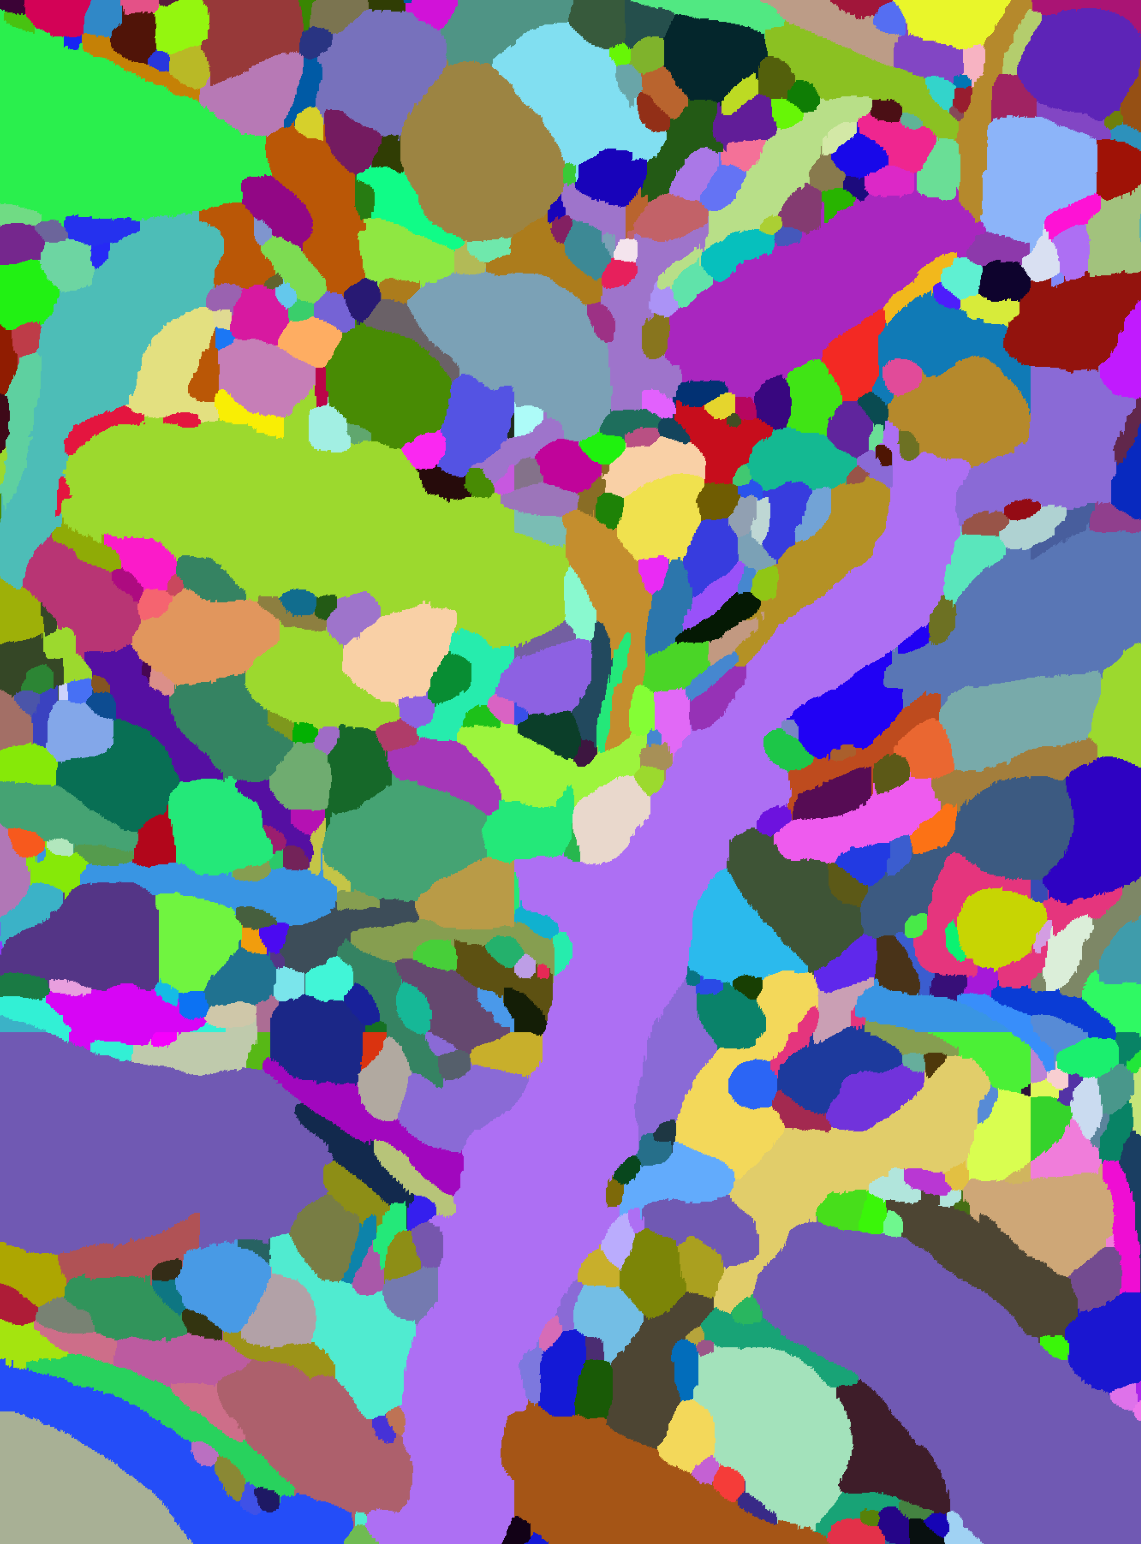
\includegraphics[width=0.24\linewidth]{./figures/methods/multicut_input.png}}
		\subfloat[]{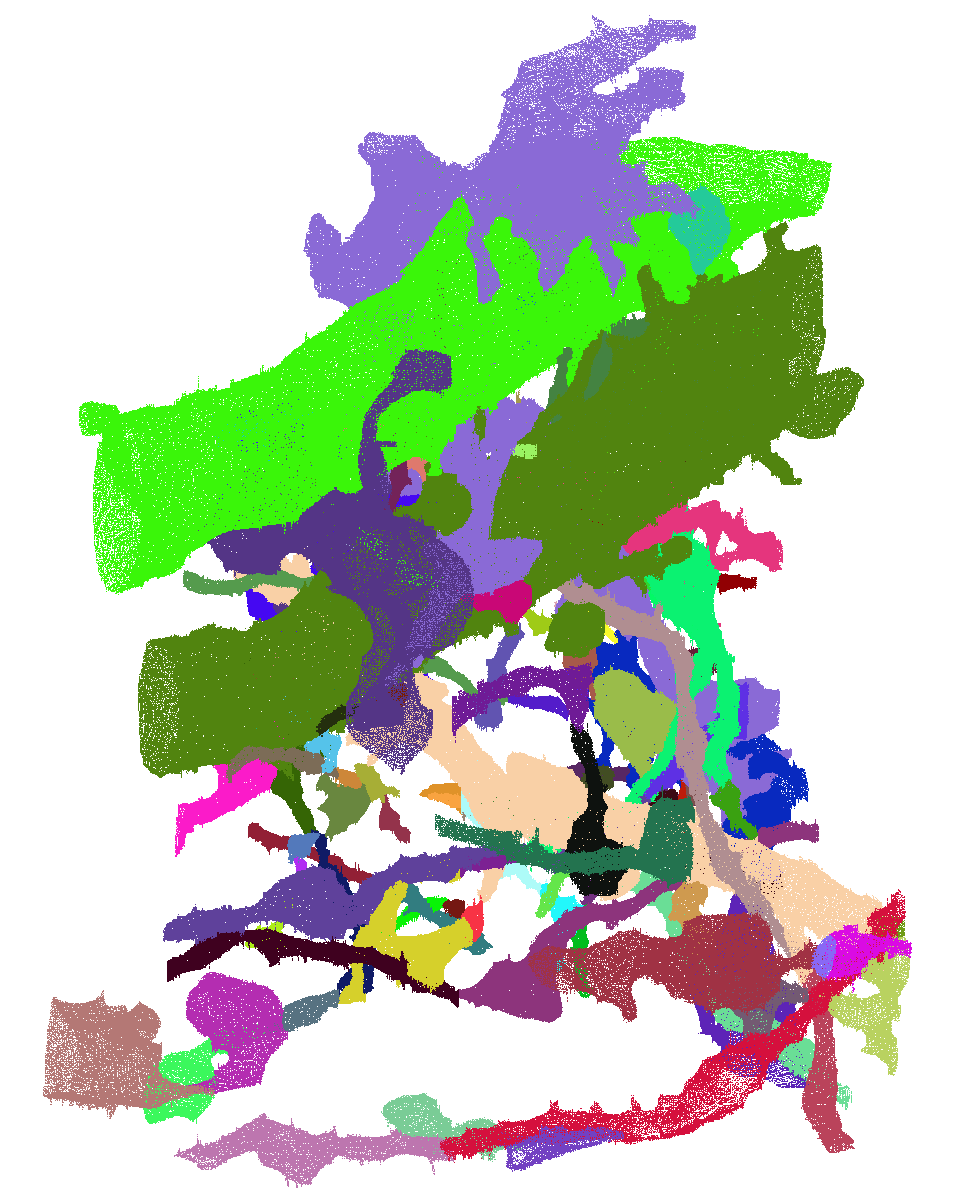
\includegraphics[width=0.24\linewidth]{./figures/methods/pre-multicut.png}}
		\subfloat[]{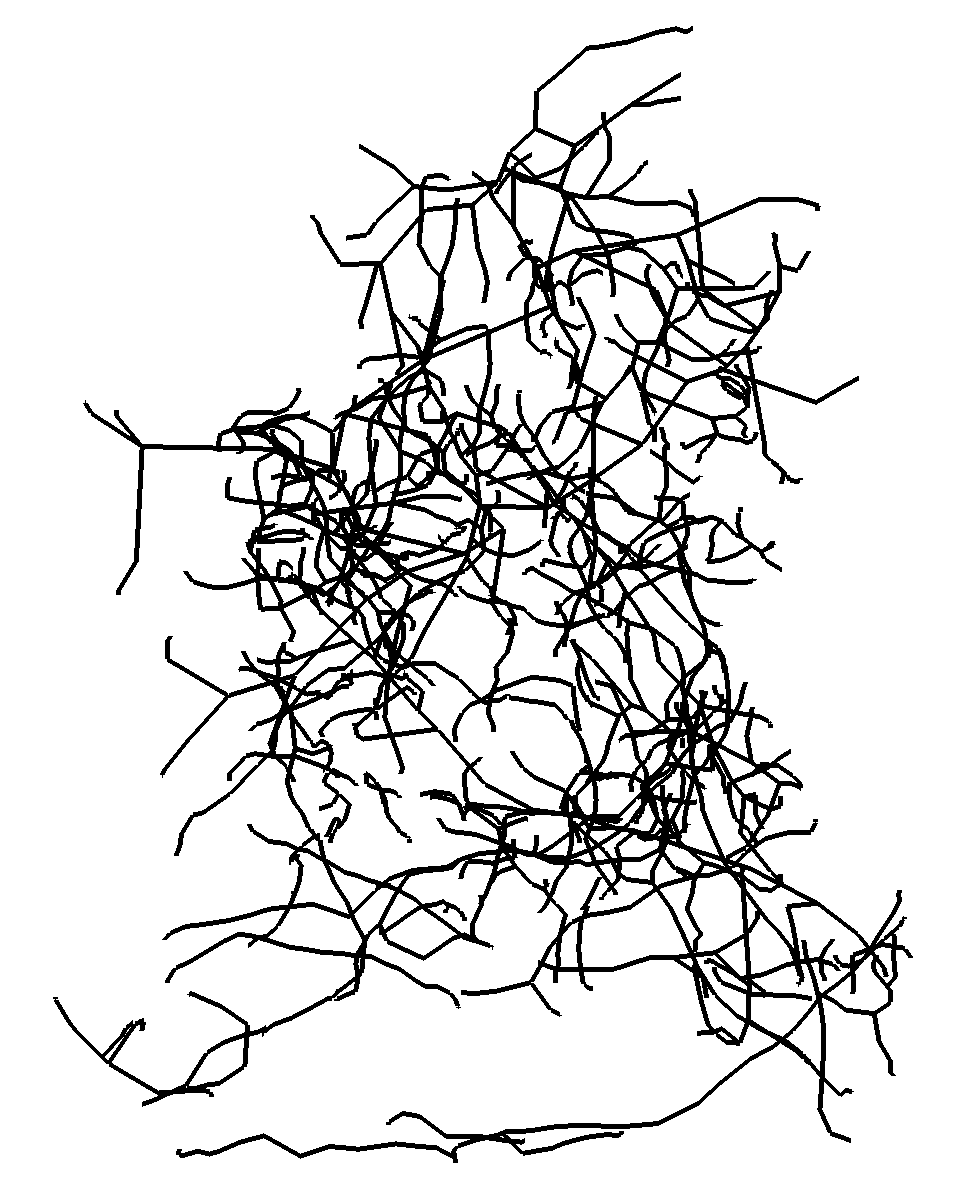
\includegraphics[width=0.24\linewidth]{./figures/methods/multicut-graph.png}}
		\subfloat[]{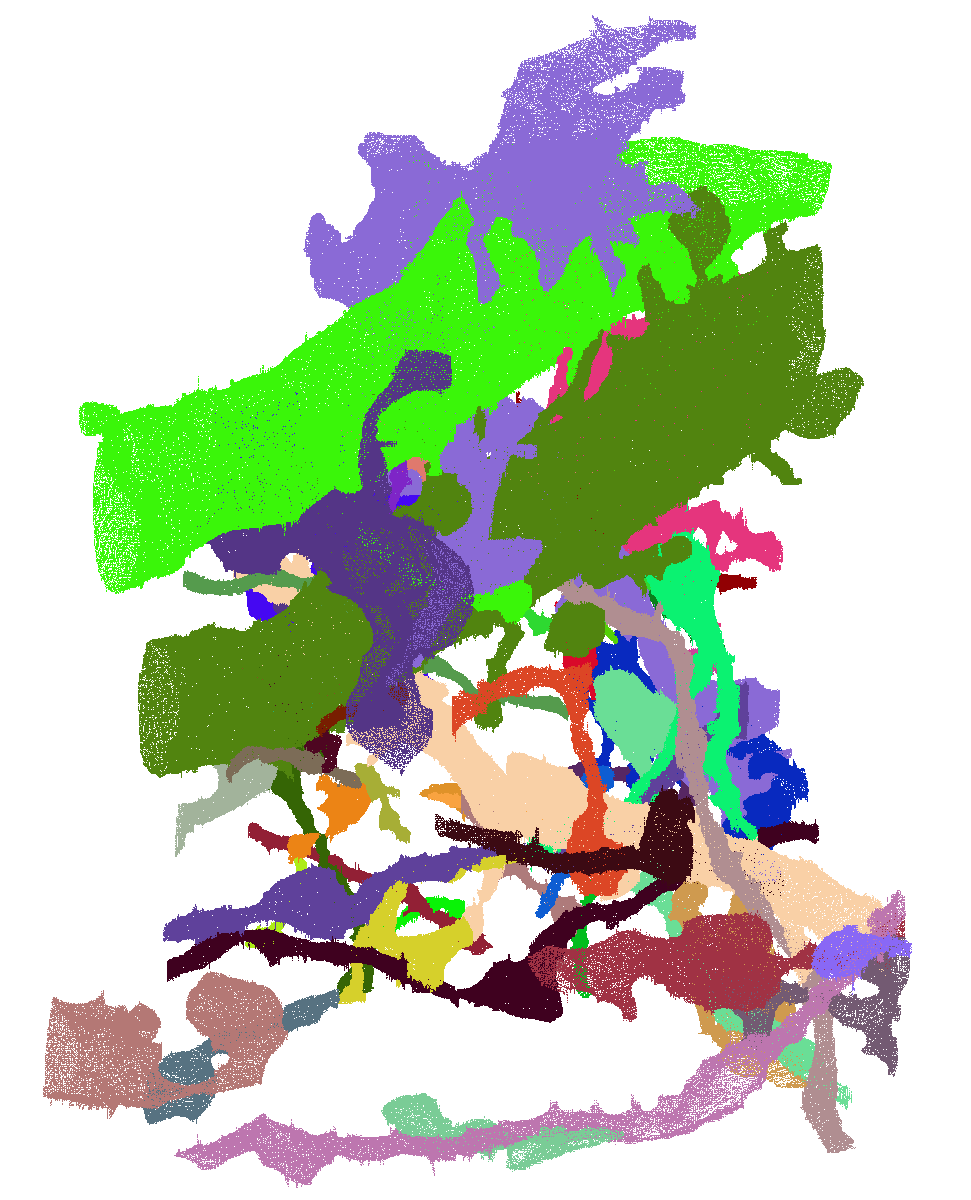
\includegraphics[width=0.24\linewidth]{./figures/methods/post-multicut.png}}
	\end{center}
	\caption{Outline of our approach, from left to right: result of the pixel-based segmentation and agglomeration algorithm; segments of several neurons from the initial segmentation; extracted skeletonized network of those segments; improved 3D reconstruction of the selected segments after graph construction and partitioning with constraints.}
	\label{fig:overview}
\end{figure*}

There are two types of errors that can occur in connectomics segmentations: \textit{split errors} and \textit{merge errors}. 
In a split error, two segments should have been merged into one neuronal process. 
In a merge error, one segment corresponds to more than one neuron.
Generally, it is much more difficult to correct merge errors than to correct split errors,
as the space of possible split proposals grows quickly~\cite{parag2015properties}.
Thus, most reconstruction approaches are tuned towards over-segmentation with many more split than merge errors. 
Our method takes as input over-segmentations of EM image volumes generated by scalable, state-of-the-art connectomics reconstruction pipelines (Sec.~\ref{sec:neuroproof}). 
Our goal is to identify locations of split errors and merge the corresponding segments automatically.

From the input segmentation we generate a graph $G$ with nodes $N$ and edges $E$ with weights $w_e$. 
The nodes correspond to labeled segments from the segmentation.
There are edges between all nodes that we consider as merge candidates.
Ideally, our graph has edges corresponding to all of the segments that were erroneously split. 
To compute this graph we generate a skeleton for every segment in the pixel-based segmentation (Fig.~\ref{fig:overview}). 
The skeletonized 3D network is a simplified representation of the overall branching structure of the neurons. 
From these skeletons we identify potential merge locations and produce the corresponding edges for the graph. 
To find actual merges we run a classification CNN to generate edge weights corresponding to merge probabilities.
We formulate our graph partitioning problem as a multicut problem to segment the nodes into correct neuronal processes. 
We will now discuss the three major components to our framework (graph creation, edge weight assignment, and graph partitioning) in more detail.

\subsection{Node Generation}
%\subsubsection{Node Generation}
\label{sec:skeletonization}

The simplest node generation strategy creates one node for every unique segment label in the input volume. 
However, some of the labels in the volume correspond to very small structures that are likely the result of segmentation errors, typically in regions with noisy raw image data. 
It is difficult to extract useful shape features from these segments because of their small, often random, shape. 
We prune these nodes from the graph by removing all segments with fewer than a threshold $t_{seg} = 20,000$ voxels. 
This removes on average \TODO{XX}\% of the segments in our  datasets (Sec.~\ref{sec:dataset}), leaving us with around $\TODO{XX}$ nodes per dataset (\TODO{X nodes per micrometer}). 
Despite the large number of segments, these regions only take up \TODO{XX}\% of the total volume on average.
We provide further analysis of this strategy in the supplemental material. 

\subsection{Edge Generation}

\begin{figure}[t]
	\centering
	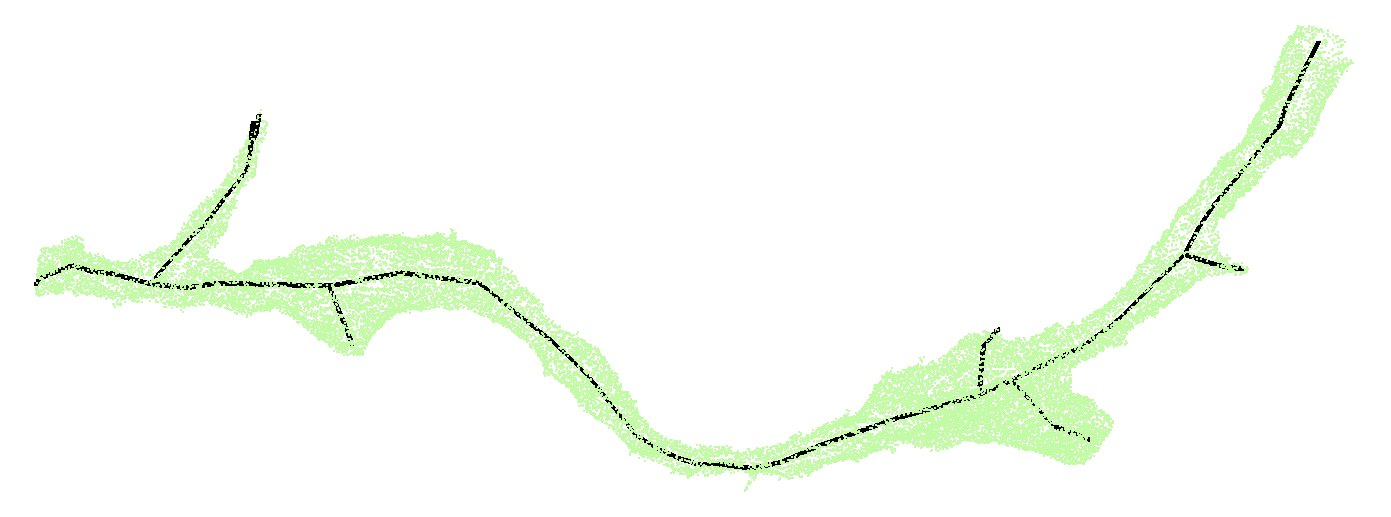
\includegraphics[width=0.45\linewidth]{./figures/skeleton1.png}
	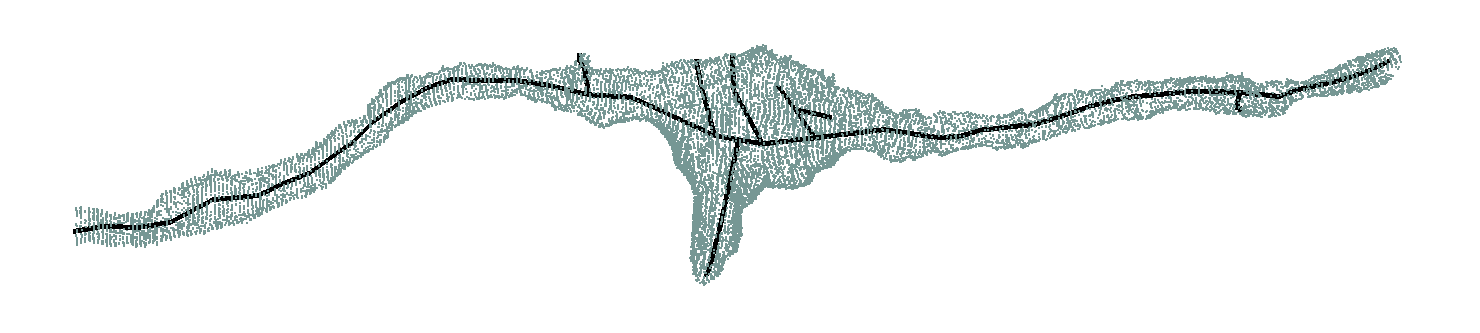
\includegraphics[width=0.45\linewidth]{./figures/skeleton2.png}
	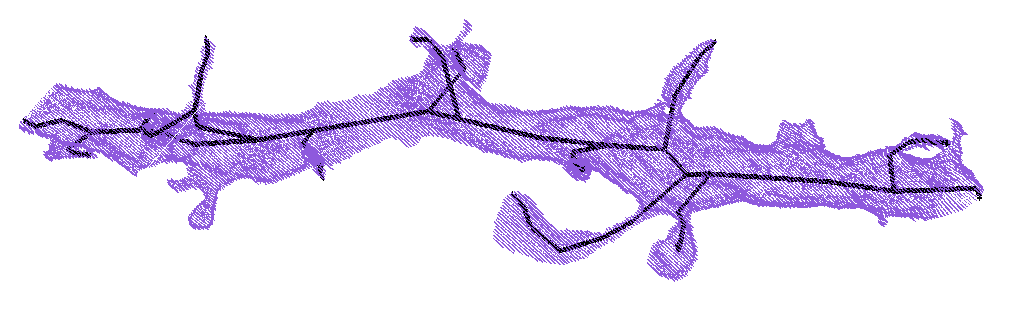
\includegraphics[width=0.45\linewidth]{./figures/skeleton3.png}
	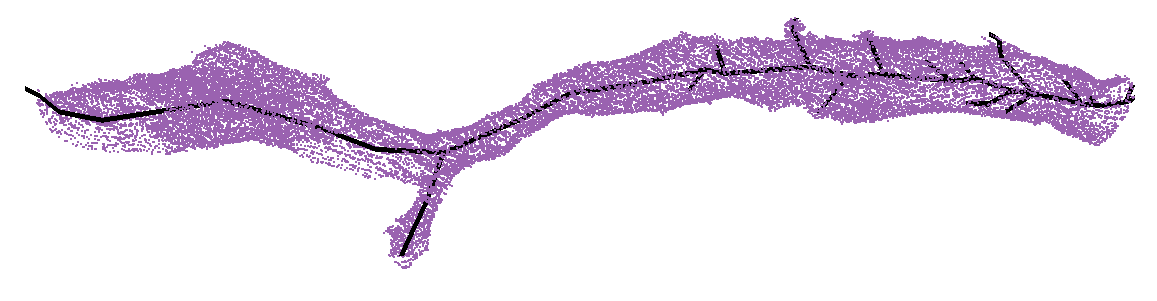
\includegraphics[width=0.45\linewidth]{./figures/skeleton4.png}
	\caption{Example skeletons (in black) extracted from segments using a variant of the TEASER algorithm.}
	\label{fig:skeletonization}
\end{figure}

A typical approach for generating edges produces one between all adjacent segments. Two segments $l_1$ and $l_2$ are considered adjacent if there is a pair of adjacent voxels with one labeled $l_1$ and the other labeled $l_2$.
For example, pixel-based agglomeration methods such as mean agglomeration~\cite{lee2017superhuman} or waterz~\cite{funke2017deep} consider all pairs of adjacent segments for merging.
However, this method produces too many edges in the graph for graph-based optimization approaches. 
We identify a smaller number of pairs of segments to consider as graph edges using the following approach.

First, we extract a skeleton from each segment in the label volume using a variant~\cite{zhao2014automatic} of the TEASER algorithm~\cite{sato2000teasar}. 
This skeletonization algorithm repeatedly uses Dijkstra's algorithm to find the farthest voxel from a seed location. 
Since this algorithm is non-linear in the number of voxels, we downsample the datasets so that there are voxel samples every $\SI{30}{\nano\meter}$ in each dimension.
Empirically, this reduced the running time for skeletonization by $\TODO{XX\%}$, with minimal reduction in skeleton accuracy ($\TODO{XX\%}$ fewer branches). 
Fig.~\ref{fig:skeletonization} shows three examples of extracted skeletons (in black). 
These skeletons consist of a sequence of \textit{joints}, i.e., locations that are locally a maximum distance from the segment boundary, with line segments connecting successive joints. 
We refer to joints that have only one connected neighbor as \textit{endpoints}. 
We find that approximately \TODO{XX\%} of the segments that are erroneously split have nearby endpoints  (Fig.~\ref{fig:merge_candidates}). 
We make use of this fact to find merge candidates with the following two-pass pruning algorithm.

In the first pass, we iterate over all endpoints $e$ belonging to a segment $S$ and create a set of segments $\mathbb{S}_e^\prime$ that includes all labels that are within $t_{low}$ voxels from $e$.
Elements of $\mathbb{S}_e^\prime$ are candidates for merging. 
However, this first pass often leads to too many candidates, requiring an additional pass for further pruning. 
In the second pass, we consider all of the segments in $\mathbb{S}_e^\prime$ for every endpoint $e$. 
If a segment $S^\prime \in \mathbb{S}_e^\prime$ has an endpoint within $t_{high}$ voxels of $e$, the segment $S$ and $S^\prime$ are considered for merging. 
We store the midpoints between the two endpoints as the center of the potential merge in the set $\mathbb{S}_c$. 
This algorithm produces a set of segments to consider for merging. Only these pairs have a corresponding edge in the constructed graph.

\subsection{Edge Weights Assignment}
\label{sec:edge-weights}
We assign edge weights $w_e$ to each edge where the weight corresponds to the probability that two nodes belong to the same neuron.
We train a 3D CNN classifier to learn from the manually labeled oversegmentation input volume (Sec.~\ref{sec:dataset}).
If the probability that the nodes belong to the same neuron is $p_e$, the edge weight $w_e = \log{\frac{p_e}{1 - p_e}} + \log{\frac{1 - \beta}{\beta}}$, where $\beta$ is a tunable parameter that encourages over- or under-segmentation.

\subsubsection{Classifier Input}

We extract a cubic region of interest (ROI) around each endpoint $e$ in $\mathbb{S}_c$ as input to the CNN. 
The CNN receives three input channels for every voxel in the ROI around segments $l_1$ and $l_2$. 
The input in all of the channels is in the range $\{-0.5, 0.5\}$. 
The first channel is $0.5$ only if the corresponding voxel has label $l_1$. 
The second channel is $0.5$ only if the corresponding voxel has label $l_2$. 
The third channel is $0.5$ if the corresponding voxel is either $l_1$ or $l_2$.
We do not use the raw EM image information to avoid the need to retrain the network on datasets that have been stained differently or imaged at different resolution. 
This reduces the need for generating costly manually-labeled ground truth. 

\begin{figure}[t]
	\centering
	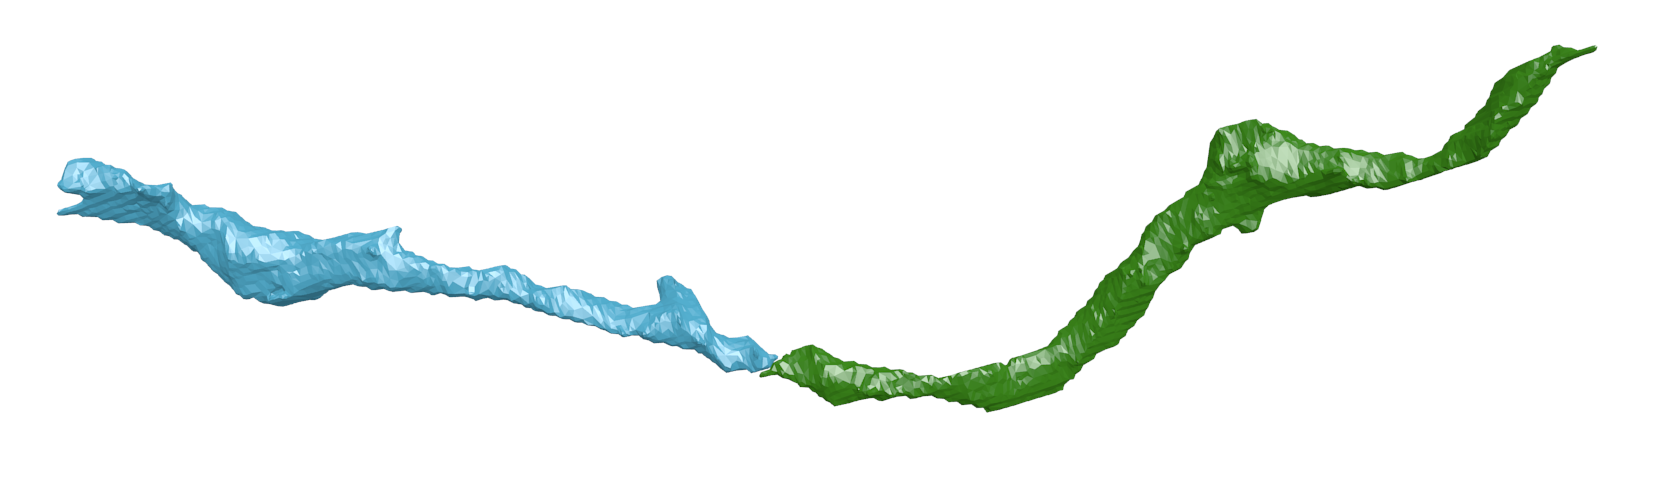
\includegraphics[width=0.32\linewidth]{./figures/split_error1.png}
	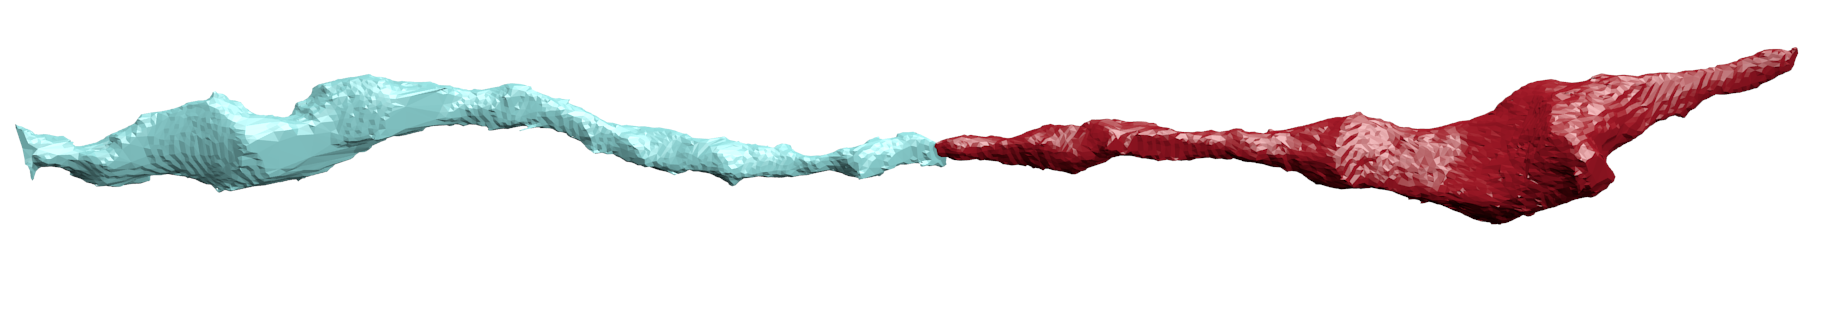
\includegraphics[width=0.32\linewidth]{./figures/split_error2.png}		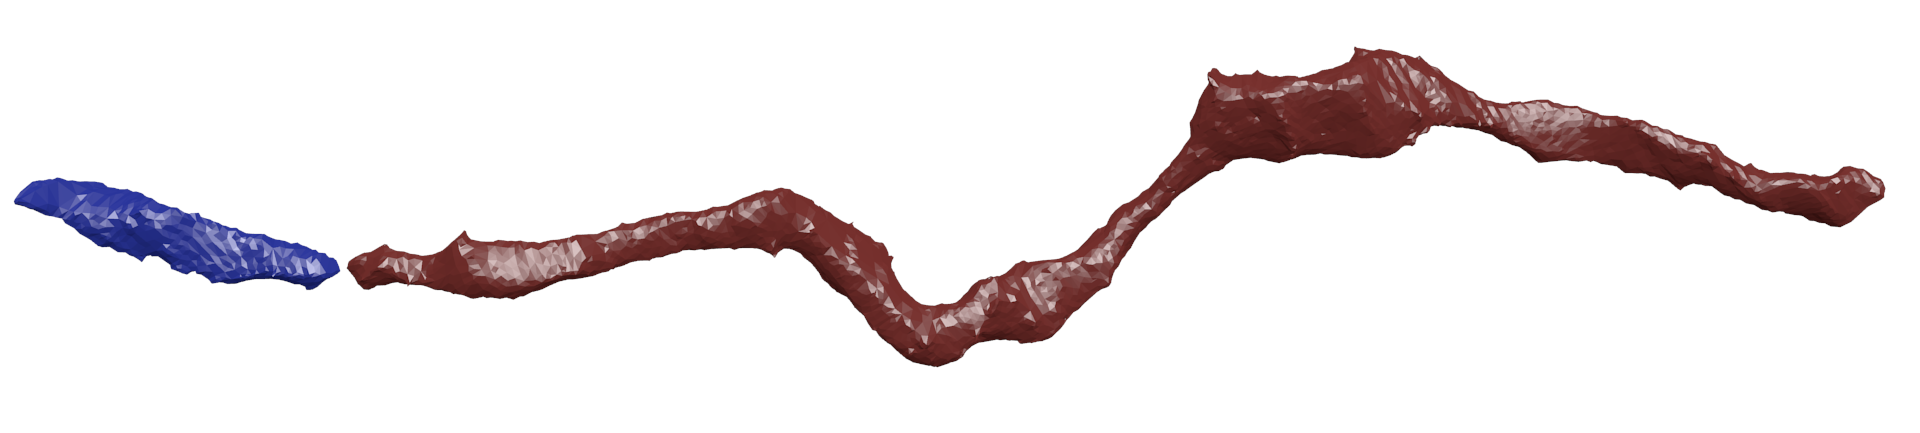
\includegraphics[width=0.32\linewidth]{./figures/split_error3.png}
	\caption{Three erroneously split segments.}
	\label{fig:merge_candidates}
\end{figure}

\subsubsection{Network Architecture \& Training}

We use \textit{VGG-style} blocks as presented by Chatfield et al.~\cite{chatfield2014return}. 
Each blocks consists of two double convolutions with filter size $3\times3\times3$ followed by a max pooling step. 
There are three layers of these blocks. 
The first two max pooling layers are anisotropic with pooling only in the $x$ and $y$ dimensions. 
The output of this final pooling step is flattened into a 1D vector that is input into two fully connected layers. 
The final layer produces probabilities with a sigmoid activation function~\cite{funahashi1989approximate}. 
All of the other activation functions are LeakyReLU~\cite{maas2013rectifier}.

For training we use a stochastic gradient descent optimizer with Nesterov's accelerated gradient~\cite{nesterov1983method}. 
We employ dropouts of $0.2$ after every pooling layer and the first dense layer, and a dropout of $0.5$ after the final dense layer to prevent overfitting. 
We discuss all other network parameters in Sec.~\ref{sec:network-parameters}.

\subsection{Graph Clustering}

After constructing the 3D graph we seek to partition the graph into labels where every label corresponds to a neuronal process. 
We formulate this graph partitioning problem as a multicut problem.
There are two primary benefits to using a multicut formulation. 
First, the number of segments in the final graph is not predetermined but depends on the input graph itself. 
Second, this minimization produces globally consistent solutions (i.e. a boundary remains if and only if the two corresponding nodes belong to unique segments).

We apply the algorithms of Keuper et al.~\cite{keuper2015efficient} to produce a feasible solution to the multicut problem using greedy additive edge contraction.
Following their example, we employ the generalized ``lifted'' multicut formulation.
Traditional multicut solutions only consider the probabilities that two adjacent nodes belong to the same segment. 
In the ``lifted'' extension to the problem, we can penalize non-adjacent nodes that belong to different segments. 
These penalties between non-adjacent nodes are called ``lifted'' edges. 
Ideally these ``lifted'' weights represent the probability that two nodes belong to the same neuron given all such possible paths in the graph between the nodes.
However, determining such probabilities is computationally expensive.
We approximate these probabilities by finding the maximal probable path between any two nodes using Dijkstra's algorithm~\cite{keuper2015efficient}.
Since our graphs are sufficiently small, we can generate ``lifted'' edges between all pairs of nodes. 

\subsubsection{Post-processing}

By reformulating the segmentation problem as a graph partitioning one, we can enforce some global constraints on our result based on the underlying biology.
Traditional hierarchical clustering algorithms do not rely on such constraints but consider local decisions independently.
We enforce a global constraint that neurons are tree-structured and should not contain cycles. 
The multicut problems returns a series of ``collapsed'' edges between nodes that belong to the same neuron.
We iterate over these edges in order of the probability of merge generated by our CNN. 
We ``collapse'' an edge only if it does not create a cycle in the graph.
